\subsection{Finaler Trainingsvorgang}
Im vorherigen Abschnitt wurde der Versuch unternommen, optimale Trainingsparameter zu ermittelt, in dem eine Reihe von Testtrainingsdurchläufen ausgeführt wurde. Anschließend wurde ein verlängertes Trainingsvorgang mit diesen Parametern durchgeführt, wodurch schlechte Werte für die Belohnungen der Agenten erreicht wurden.   

Da nicht das gewünschte Ergebnis erzielt wurde, wurden weitere Testtrainingsvorgänge durchgeführt. Es wurde festgestellt, dass bei einer Verringerung der Lernrate auf $1e-4$ und einer Erhöhung der Batchgröße auf $64$ bessere Ergebnisse erzielt werden können. Zusätzlich wird die Anzahl der Trainingsschritte auf \Fachbegriff{1e6} erhöht. Mit diesen Parametern wird nun ein finales, verlängertes Training durchgeführt, das zu einem verbesserten Lernvorgang führen soll. In den folgenden Diagrammen sind die Resultate dieses Trainingsvorgangs abgebildet.

Im Vergleich zum Basistraining wurden unmittelbar leicht verbesserte Ergebnisse für alle drei verwendeten Metriken erzeugt. Durch die Verlängerung des Trainings konnte weiterhin ein leichter, stetiger Anstieg bei der Belohnungsfunktion und ein leichter, stetiger Abstieg für die Entropie und den Value Loss ausgenutzt werden, um insgesamt bessere Ergebnisse zu erlangen.
Die maximale Belohnung beträgt im Basistraining 5,241 und im finalen Training 5,429. Die Gesamtbelohnung pro Episode wurde damit um ca. 3,6\% gesteigert. Der minimale Value Loss wurde von 0,073 auf 0,037 verbessert. Weiterhin konnte die Entropie von 1,127 auf 0,642 verringert werden.

\begin{figure}[H]
\centering
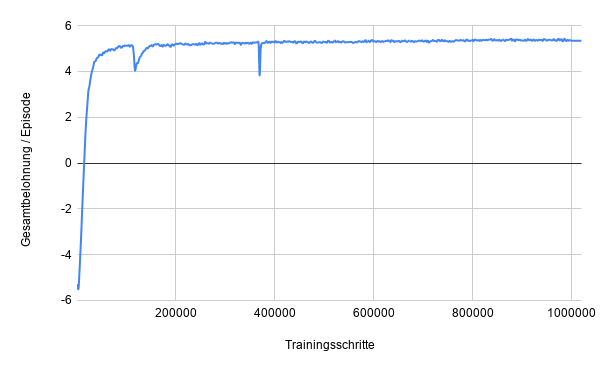
\includegraphics[scale=0.7]{images/training/final/final_rewards.png}
\caption{Akkumulierte Belohnungen im finalen Training des \inlinecode{NpcAgent}}
\label{fig:final_rewards}
\end{figure}

\begin{figure}[H]
\centering
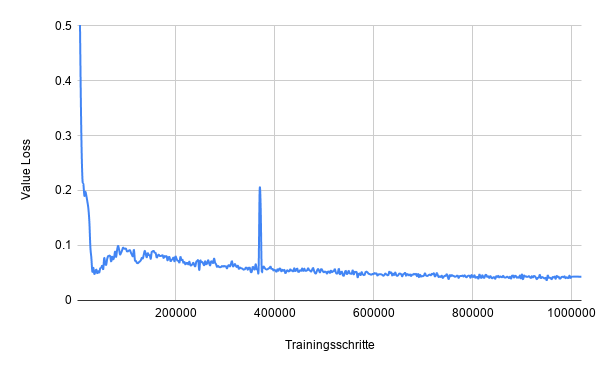
\includegraphics[scale=0.7]{images/training/final/final_loss.png}
\caption{Value Loss im finalen Training des \inlinecode{NpcAgent}}
\label{fig:final_loss-loss}
\end{figure}

\begin{figure}[H]
\centering
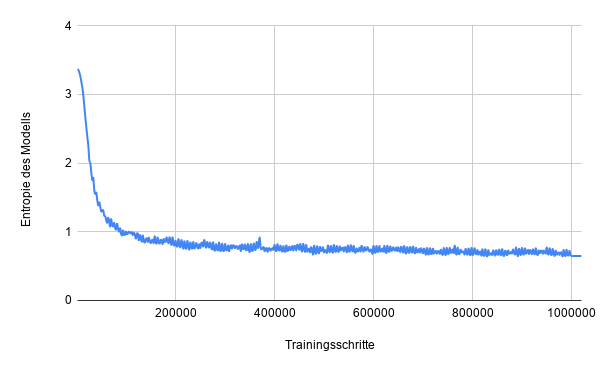
\includegraphics[scale=0.7]{images/training/final/final_entropy.png}
\caption{Entropieverlauf im finalen Training des \inlinecode{NpcAgent}}
\label{fig:final_entropy}
\end{figure}








\subsection{Verhalten der Agenten}\label{7_result_agent_behavior}
Durch den finalen Trainingsvorgang wurde ein Modell für die Entscheidungsfindung der NPCs erzeugt. Das Modell bestimmt das Verhalten der Agenten, das im Folgenden untersucht wird.


\subsubsection{Eindruck}
Der erste Eindruck erweckt den Anschein einer belebten Stadt, in der viele NPCs unterschiedliche Tätigkeiten ausführen. Es wirkt lebendig, da in allen Bereichen des Dorfes NPCs umherlaufen. Damit wird zunächst genau der Eindruck erzielt, der vermittelt werden soll. Dem Anschein nach befindet sich der Spieler in einer belebten Welt, in der eine Vielzahl von Agenten ihrem persönlichen Leben nachgehen. Durch die Betrachtung der Informationen im UI ist weiterhin auffällig, dass unterschiedliche Aktionen ausgeführt werden.


\subsubsection{Auswahl von Aktionen aufgrund von Bedürfnissen}
Über einen längeren Zeitraum wurden mehrere Agenten näher betrachtet. Dabei wurde für jede Aktion, die sie ausgeführt haben, auf ihre Bedürfnisse geachtet, um zu bewerten, ob die Entscheidungen der Agenten sinnvoll sind. Dabei wurde festgestellt, dass die Agenten in fast allen Fällen eine Entscheidung treffen, die für einen Beobachter unter Berücksichtigung der Bedürfnisse des Agenten sinnvoll erscheinen. Aus diesen Beobachtungen kann gefolgert werden, dass die Agenten erfolgreich gelernt, haben, aufgrund ihrer Bedürfnisse Entscheidungen zu treffen, die diese befriedigen. In dem überwiegenden Großteil der Beobachtungen wählten die Agenten Aktionen für das Bedürfnis, das den niedrigsten Bedürfniswert hatte.
Im \inlinecode{NeedCycleHandler} wurden für die Bedürfnisse \Fachbegriff{Hunger}, \Fachbegriff{Durst}, \Fachbegriff{Bildung}, \Fachbegriff{Kommunikation} und \Fachbegriff{Glauben} Konstanten festgelegt. Diese bestimmen den Zyklus der Bedürfnisse und damit die Steigung der Bedürfnisfunktion und die Dauer bis zum Erreichen eines kritischen Bedürfnislevels. In den Beobachtungen aus der Dorfsimulation spiegelt sich die unterschiedliche Dauer der Zyklen wider. Die verschiedenen Bedürfnisse werden in unterschiedlichen zeitlichen Abständen befriedigt. Die definierten Konstanten decken sich dabei mit dem Ausführungsrhytmus der jeweiligen Aktionen. Das Glaubensbedürfnis erreicht zum Beispiel nach drei Tagen den Wert $0$. Etwa alle drei Tage wird das Bedürfnis gestillt.

Im Gegensatz zu den genannten Basisbedürfnissen kann weiterhin festgestellt werden, dass die NPCs in regelmäßigen Abständen arbeiten und schlafen. Das ist sinnvoll, weil das Schlaf- und das Arbeitsbedürfnis direkt von der simulierten Zeit des Dorfes abhängt. Dadurch entsteht für die Agenten ein grober Tagesablauf. Zusätzlich wurde die Beobachtung aufgestellt, dass die Agenten relativ genau ein mal pro Tag schlafen und arbeiten.



\subsubsection{Beitrag der Attribute zur Entscheidungsfindung}
Während der Entwicklung der Simulation kam es häufig dazu, dass Agenten bestimmte Aktionen bevorzugt haben, da für diese die höchste Belohnung erwartet wurde. Das ist besonders für \Fachbegriff{Recreation}-Aktionen relevant, da diese Aktionen alle dasselbe Bedürfnis befriedigen. Um das Problem zu umgehen, wurden die Belohnungen der Aktionen von den Attributen der Agenten abhängig gemacht. Weiterhin ist der Beruf des Agenten ausschlaggebend für die Attribute der Agenten. In der folgenden Abbildung ist die resultierende Verteilung der Attribute in Abhängigkeit von den Berufen zu sehen:

\begin{figure}[H]
\centering
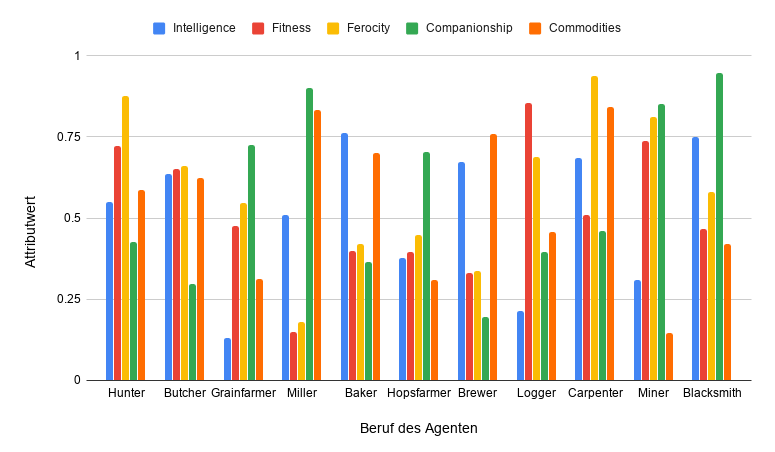
\includegraphics[scale=0.6]{images/training/attribute_job_results.png}
\caption{Verteilung der Attribute und Berufe der Agenten}
\label{fig:attribute_job_results}
\end{figure}

Weiterhin wird in der folgenden Grafik \ref{fig:attribute_action_results} die durchschnittlichen Höhe der Attribute von Agenten für Recreation-Aktionen dargestellt. In einer Tabelle werden zusätzlich die jeweiligen Attribute festgehalten, die für die Belohnungen der Recreation-Aktionen genutzt werden. Dafür werden die Identifier für die Aktionen und Attribute genutzt. Die Belohnungen für Attribute können invertiert werden, sodass ein hohes Attribut für die Aktion zu einer Strafe führt. 

\begin{figure}[H]
\centering
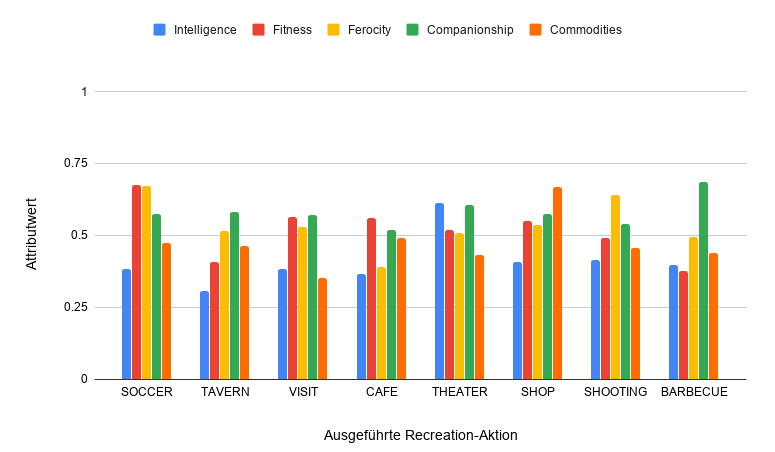
\includegraphics[scale=0.6]{images/training/attribute_action_results.png}
\caption{Verteilung der Attribute und Berufe der Agenten}
\label{fig:attribute_action_results}
\end{figure}

\smallskip
\begin{table}[H]
\begin{tabular} {|  p{5cm}  |  p{10.6cm}  |} \hline
\textbf{Aktion} & \textbf{Attribute} \\ \hline
RECREATION\_SOCCER & ATT\_FITNESS, ATT\_FEROCITY. \\ \hline
RECREATION\_TAVERN & ATT\_INTELLIGENCE (invertiert), ATT\_FITNESS (invertiert). \\ \hline
RECREATION\_VISIT & ATT\_COMPANIONSHIP, ATT\_COMMODITIES (invertiert). \\ \hline
RECREATION\_THEATER & ATT\_INTELLIGENCE. \\ \hline
RECREATION\_CAFE & ATT\_COMPANIONSHIP, ATT\_FEROCITY (invertiert). \\ \hline
RECREATION\_SHOP & ATT\_COMMODITIES, ATT\_FEROCITY (invertiert). \\ \hline
RECREATION\_SHOOTING & ATT\_FEROCITY, ATT\_COMPANIONSHIP (invertiert). \\ \hline
RECREATION\_BARBECUE & ATT\_COMPANIONSHIP, ATT\_FITNESS (invertiert). \\ \hline

\end{tabular}
\caption{Beeinflussing der Belohnungen von Recreation-Aktionen durch Attribute}
\label{tab:recreation_actions_attributes}
\end{table}

Die Verteilung der Attribute deckt sich ungefähr mit den Attributboni, die in der obigen Tabelle dargestellt werden. Dadurch wird gezeigt, dass die Attribute der Agenten bei der Wahl der Recreation-Aktion eine Rolle spielen. Agenten mit Attributen, die einen Bonus für die Belohnung einer bestimmten Aktion zur Folge haben, führen diese Aktion also statistisch gesehen häufiger aus als andere Aktionen. Die im Abschnitt \ref{agents_rewards} angesprochene Einteilung der Agenten in Gruppen wurde daher erreicht. Auch durch simple Beobachtungen lässt sich diese Eigenschaft überprüfen; beispielsweise trifft man in der Taverne tatsächlich häufiger Agenten mit einem niedrigen Intelligenzlevel an, wie etwa Bauern oder Holzarbeiter.




\subsubsection{Tagesablauf und Bedürfnisverlauf}
Die durchschnittlichen Bedürfnisse der Agenten wurden über einen Zeitraum von 100 Simulationstagen beobachtet und zu bestimmten Tageszeiten festgehalten. Schließlich wurden von allen Agenten die mittleren Bedürfniswerte für bestimmte Tageszeiten berechnet, wie in Abschnitt \ref{village_logging} beschrieben. Daraus hat sich der folgende Bedürfnisverlauf ergeben:

\begin{figure}[H]
\centering
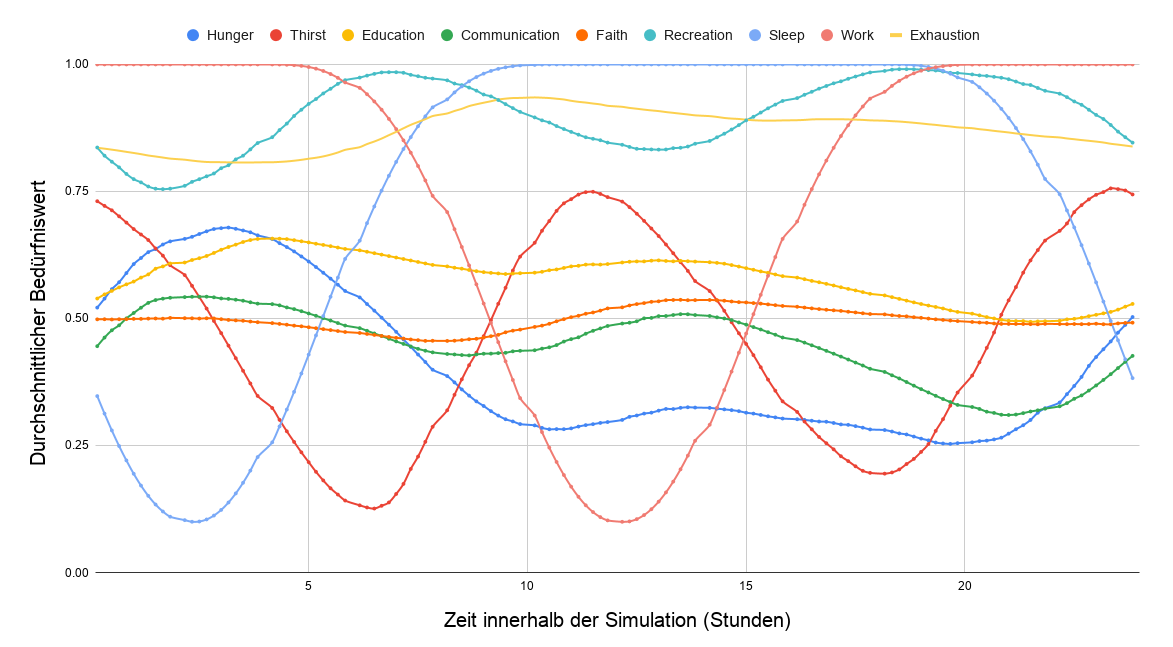
\includegraphics[scale=0.4]{images/training/reinforcement_needs_day_cycle.png}
\caption{\ac{reinforcement_learning}-Ansatz, Verlauf der durchschnittlichen Bedürfniswerte}
\label{fig:reinforcement_needs_day_cycle}
\end{figure}

Zum Verlauf der Bedürfnisse wird angemerkt, dass die Variable \inlinecode{\_rythmVariation} zur Erzeugung eines Offsetes zwischen Agenten im \inlinecode{NeedCycleHandler} (siehe Abschnitt \ref{npc_needs_architecture}) für die Aufzeichnung der Daten deaktiviert wurde. Dadurch sollen Unterschiede zwischen den Agenten eliminiert werden. Der gezeigte Verlauf ist zwar repräsentativ für alle Agenten, normalerweise würde für jeden einzelnen Agenten jedoch eine horizontale Verschiebung der Bedürfnisse durch die Verwendung des Offsets entstehen.
Weiterhin entsprechen die gewählten Schlaf- und Arbeitszeiten nicht unbedingt dem durchschnittlichen Menschen unserer heutigen Gesellschaft, da bei der Entwicklunge der Zyklen mit normalisierten Float-Werten zwischen 0 und 1 gearbeitet wurde. Die Schlaffunktion erreicht ihr Minimum erst um etwa 2:30 Uhr nachts. Für das Verhalten des Agenten spielt dies jedoch keine Rolle. Durch eine simple Transformation könnten die Zyklen verschoben werden, in dieser Analyse werden sie jedoch in der vorliegenden Form akzeptiert.

Weiterhin kann man feststellen, dass sich die Bedürfnisse nicht zufällig entwickeln, sondern von der jeweiligen Tageszeit abhängen. Es sind Kurven entstanden, die Hinweise darauf geben, wann Bedürfnisse befriedigt werden.

Die Hungerfunktion wurde so gewählt, dass sie nach einem halben Tag den Wert $0$ erreicht. Am Verlauf des Hungers ist zu erkennen, dass das Bedürfnis in der Nacht zunächst zunimmt und dann sinkt, sobald sich die Agenten schlafen legen. Das Hungergefühl wächst dann automatisch an, weil der Agent mit der Aktion \Fachbegriff{Schlafen} beschäftigt ist. Über den Tag verteilt bleibt das Hungergefühl auf einem relativ gleichbleibenden aber akzeptablen Level. Das spricht dafür, dass die Agenten zu unterschiedlichen Zeiten essen. Ob der Agent direkt nach dem Aufwachen essen muss, hängt von den zuvor getätigten Aktionen und somit den aktuellen Bedürfnissen des Agenten ab.
Das Durstgefühl des Agenten wird hingegen von einer deutlich stärker schwankenden Funktion beschrieben, die einer Sinuskurve ähnelt. Die Durstfunktion wurde so definiert, dass sie etwa drei mal am Tag den Wert $0$ erreicht, wenn das Durstgefühl nicht gestillt wird. Tatsächlich ist an dem Graphen zu erkennen, dass die Agenten zwei mal am Tag ihr Durstgefühl stillen - nach dem Aufwachen und nach der Arbeit. Schlussfolgernd muss sich das Durstgefühl des Agenten für eine gewisse Zeit auf dem Wert $0$ befinden. Das bedeutet nicht, dass der Agent die falschen Aktionen getroffen hat - zur gleichen Zeit können mehrere Bedürfnisse den Wert $0$ annehmen. Die Belohnungen für die Bedürfnisse \Fachbegriff{Arbeit} und \Fachbegriff{Schlaf} sind darüber hinaus deutlich höher als die Belohnungen für weitere Bedürfnisse. Das bedeutet, dass ein Agent, der hungrig und durstig ist, sich trotzdem für die Aktion \Fachbegriff{Arbeit} entscheiden würde, wenn das entsprechende Bedürfnis klein genug ist. Die Belohnungen wurden so gewählt, um einen gleichbleibenden Tagesablauf des Agenten zu gewährleisten. Weiterhin haben alle Aktionen eine gewisse Dauer. Erst nachdem die Dauer der Aktion vorüber ist, kann eine weitere Aktion ausgeführt werden, die ein zwischenzeitlich auf den Wert $0$ gesunkenes Bedürfnis befriedigen soll. Solange die erste Aktion und selbst die zweite Aktion noch ausgeführt wird, kann dieses Bedürfnis auf dem Wert $0$ stagnieren. Erst nachdem die zweite Aktion beendet wurde, wird das Bedürfnis aufgefüllt.
Es ist daher logisch, dass der Agent nur zwei mal am Tag seinen Durst stillt, obwohl das Bedürfnis theoretisch drei mal am Tag auf den Wert $0$ sinkt, denn die Ausführung der \Fachbegriff{richtigen} Aktion ist nicht immer möglich, etwa, weil der Agent mit anderen Dingen beschäftigt ist.

Die Bedürfnisse nach Bildung und Glauben bleiben über den gesamten Tag auf einem relativen ähnlichen Level. Das liegt daran, dass erst nach 1,9 Tagen das Bildungs- und erst nach drei Tagen das Glaubensbedürfnis auf den Wert $0$ abgefallen ist. Da Exponentialfunktionen für die Berechnung der Bedürfnisse verwendet wurden, sind die beiden Bedürfnisse für den Großteil dieser Zeit auf einem hohen Level in der Nähe des Wertes $1$. Beide Bedürfnisse verzeichnen einen leichten Anstieg um etwa 10:00 Uhr, was darauf hindeutet, dass Agenten um diese Zeit häufig ihr Glaubens- und Bildungsbedürfnis befriedigen. Weiterhin hat das Bildungsbedürfnis einen leichten Anstieg um etwa 22:00 Uhr.

Das Bedürfnis nach Kommunikation verhält sich auf ähnlich wie das Bedürfnis nach Bildung. Dieses Bedürfnis sinkt nach 0,95 Tagen auf den Wert $0$ ab. Besonders häufig wird es um etwa 20:30 befriedigt, nachdem der Agent von der Arbeit gekommen ist und etwas getrunken hat. Analog zu diesem Verlauf sind etwa um diese Zeit in der Simulation viele Dorfbewohner auf dem Marktplatz zu sehen, die sich treffen, um zu kommunizieren.
Die \Fachbegriff{Exhaustion} sinkt über den Tag langsam ab. Sobald die Agenten schlafen, erhöht sich das Bedürfnis automatisch wieder, da die Agenten sich erholen. Es sind keine starken Steigungen zu beobachten, die darauf hinweisen, dass sich Agenten zu bestimmten Zeiten ausruhen.

Sowohl das Schlaf- als auch das Arbeitsbedürfnis werden nicht durch die Aktionen der Agenten beeinflusst. Stattdessen hängen sie direkt von der Zeit in der Simulation ab. Sie erfüllen lediglich den Zweck, die Belohnungen der Agenten von einer Bedürfnisfunktion abhängig zu machen, die Bedürfnisse lassen sich aber nicht auffüllen. Sobald ein Agent schläft oder arbeitet, dauern die entsprechenden Aktionen so lange, dass bei der Beendigung wieder der Wert $1$ für das Bedürfnis erreicht wird. Die in der Abbildung \ref{fig:village_diagram_sleep_work_functions} dargestellten Funktionen sind in der oben zu sehenden Grafik gut wiederzuerkennen. Die Zeitpunkte der Befriedigung der weiteren Bedürfnisse hängt vom Schlaf- und Arbeitsbedürfnis indirekt ab. Durch die Etablierung dieser beiden zeitabhängigen Bedürfnisse wurde das Fundament für den weiteren Tagesablauf der Agenten gelegt. Sie bestimmen, wann der Agent Zeit für weitere Aktionen hat. Durch die hohe Dauer der Aktionen verringern sich weiterhin automatisch stark die Bedürfnisse des Agenten, sobald er arbeitet oder schläft. Es ist daher logisch und notwendig, dass ein NPC direkt nach dem Arbeiten oder Schlafen etwas trinken muss.





\subsubsection{Dauer der Aktionen}
Über einen Zeitraum von 100 Simulationstagen wurde die Dauer aller Aktionen gespeichert. Schließlich wurde aus der Menge der Dauer für eine Aktion der jeweilige Durchschnitt berechnet, wie in Abbildung \ref{fig:avereage_action_durations} zu sehen.

\begin{figure}[H]
\centering
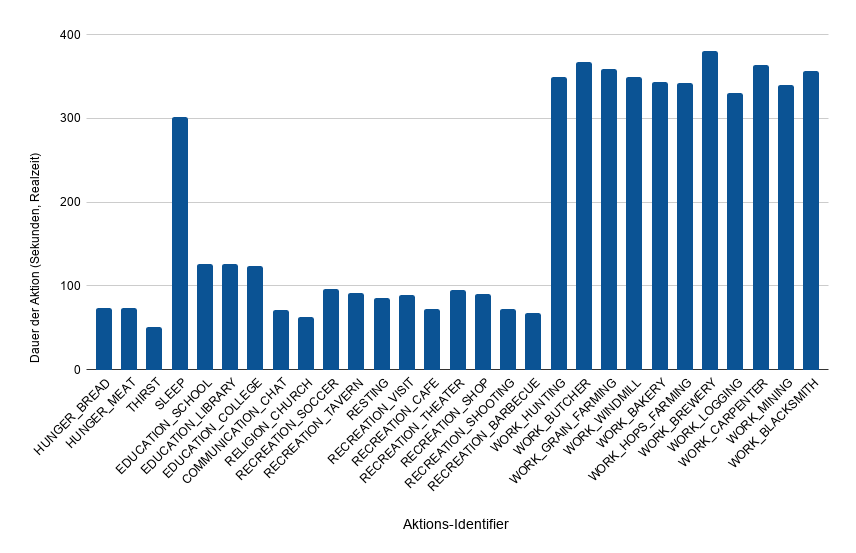
\includegraphics[scale=0.5]{images/training/avereage_action_durations.png}
\caption{Durchschnittliche Dauer der Aktionen}
\label{fig:avereage_action_durations}
\end{figure}

Die Teilaktionen der ActionPlans wurden so festgelegt, dass Aktionen, die dasselbe Bedürfnis befriedigen, möglichst gleich viel Zeit benötigen. Die Abbildung zeigt, dass die Ausführung der Recreation-Aktionen ähnlich viel Zeit braucht. Weiterhin stimmen die Dauern der beruflichen Aktionen ungefähr überein. Die in den Teilaktionen festgelegten Dauern wurden daher korrekt gewählt.

Die Festlegung der Dauern ist besonders schwierig, weil sich der Startort eines Agenten bei der Ausführung einer Aktion stets ändert. Daher variiert die benötigte Dauer, um zum Zielort zu gelangen. Die Abbildung zeigt, dass die Teilaktionen der ActionPlans gut definiert wurden, da insgesamt die gewünschten Dauern erreicht wurden.  


\subsubsection{Anzahl der Aktionen im Verhältnis}
Um einen Eindruck über die relativen Häufigkeiten der Aktionen zu erlangen, wurden über einen Zeitraum von 100 Simulationstagen die Mengen der jeweils ausgeführten Aktionen gespeichert. Dieses Verhältnis wird in der folgenden Abbildung dargestellt:
 
\begin{figure}[H]
\centering
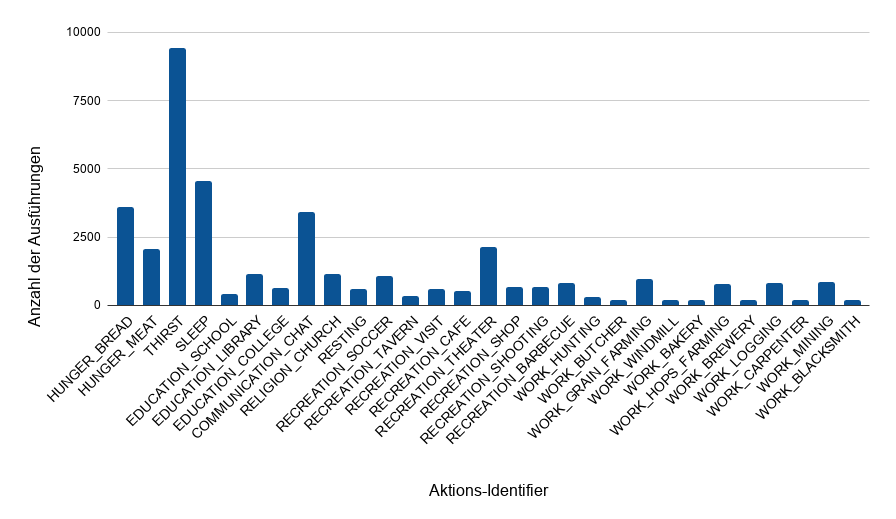
\includegraphics[scale=0.5]{images/training/actions_amounts_relation.png}
\caption{Verhältnis der Menge der ausgeführten Aktionen}
\label{fig:actions_amounts_relation}
\end{figure}

Insgesamt wurden 38.799 Aktionen von 50 Agenten ausgeführt. Im Durchschnitt hat jeder Agent also ca. 804 Aktionen insgesamt bzw. ca. 7,76 Aktionen pro Tag ausgeführt. Die jeweilige Anzahl der entsprechenden Aktionen deckt sich mit den im \inlinecode{NeedCycleHandler} festgelegten Zyklusdauern sowie den in der Abbildung \ref{fig:reinforcement_needs_day_cycle} beobachteten Verläufen. Das Bedürfnis \Fachbegriff{THIRST} wird zum Beispiel deutlich häufiger befriedigt als das Bedürfnis \Fachbegriff{FAITH}, da unterschiedliche Zyklusdauern festgelegt wurden.

Die Aktion \inlinecode{EDUCATION\_LIBRARY} wurde deutlich häufiger als andere Bildungs-Aktionen ausgeführt. Das liegt daran, dass die Altersgruppe für die Bibliothek deutlich mehr Agenten beinhaltet als die des College oder der Schule.

Auffällig ist lediglich, dass unproportional viele Agenten die Aktion \inlinecode{RECREATION\_THEATER} ausgeführt haben. Diese Anomalie könnte zum einen damit erklärt werden, dass ein Fehler im Programmcode vorliegt, oder zum anderen, dass der Trainingsvorgang nicht ideal verlaufen ist. 


\subsubsection{Maskierte Aktionen}
Weiterhin wurde die Anzahl der maskierten Aktionen untersucht. Für die Entscheidungen aller Agenten wurde dafür die Menge der maskierten Aktionen gespeichert. Da NPCS feste Berufe haben und deswegen nur eine berufliche Aktion ausführen können, beträgt die Menge der maskierten Berufsaktionen - mit Ausnahme der Aktion, die zum Job des Agenten gehört - genau der Menge der insgesamt ausgeführten Aktionen. Ähnlich verhält es sich mit den Bildungs-Aktionen, da diese vom Alter des Agenten abhängen. Alle anderen Aktionen wurden im Durchschnitt lediglich zwei Mal maskiert, was bei über 800 ausgeführten Aktionen für das Training nicht nennenswert ins Gewicht fallen sollte.